\ofsubsection{Blitzball}
%
\ofquote{"The players fight with all their strength: the fans cheer for their favorite team. They forget pain, suffering... Only the game matters! That's why Blitz has been around for so long. Least that's what I think."\\}{Wakka}\\\\
%
\accf{Blitzball} is a team sport that can be compared to water polo except that the game is played underwater, inside a large water sphere.
The water itself is imbued with magical properties to allow players to stay submerged for an extended period.
In Blitzball two opposing teams play against each other and the team which scores the most points wins.
A point is scored by shooting the ball inside the enemy goal. 
Each team consists of one goalkeeper and 2-5 players. 
Blitzball is similar to combat, except that the game is centered around controlling the ball.
The turn order is determined in the exact same way as in combat and the player who takes the first turn catches the ball after kick-off.
Each game consists of two halves, where each half consists of 10 rounds.
After finishing the first half, the teams take a break where every player fully recovers their SP.
Blitzball is played inside a 15u diameter sphere filled with water, but you can use the simplified layout shown below to illustrate games.
%
\vfill
%
\begin{figure}[h]
	\centering
	\resizebox{\columnwidth}{8cm}{%
	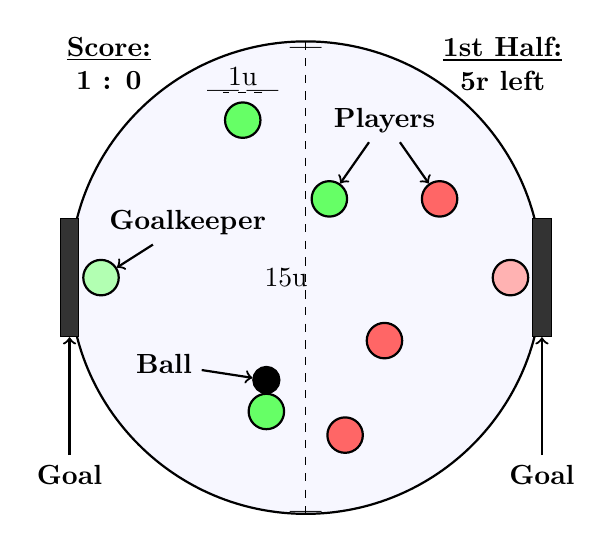
\begin{tikzpicture}[]
	\tikzstyle{test}=[thick, draw, circle, align=center]					
	\node[fill=blue!3!white, test, thick ,minimum size = 6cm](tarea)at (0,0) {};

	\node[fill=red!60!white, test,minimum size = 0.45cm](player2)at (1.7,1) {};
	\node[fill=red!60!white, test,minimum size = 0.45cm](target)at (1,-0.8) {};
	\node[fill=red!60!white, test,minimum size = 0.45cm](target)at (0.5,-2) {};

	\node[fill=green!60!white, test,minimum size = 0.45cm](target)at (-0.8,2) {};
	\node[](a1)at (-0.55,2.35) {\bf |};
	\node[](a2)at (-1.05,2.35) {\bf |};
	\node[](a2)at (-0.8,2.55) {1u};
	\draw[-, dashed](-0.55,2.35) -- (-1.05,2.35);
	
	\node[fill=green!60!white, test,minimum size = 0.45cm](player)at (0.3,1) {};
	\node[fill=green!60!white, test,minimum size = 0.45cm](target)at (-0.5,-1.7) {};
	\node[fill=black, test,minimum size = 0.1cm](ball)at (-0.5,-1.3) {};		
	\node[](tball)at (-1.8,-1.1) {\bf Ball};
	\node[](tplayer)at (1,2) {\bf Players};
	\draw[->, thick](tball) -- (ball);
	\draw[->, thick](tplayer) -- (player);
	\draw[->, thick](tplayer) -- (player2);
	
	\node[](tgk)at (-1.5,0.7) {\bf Goalkeeper};
	\node[](tgoal)at (-3,-2.5) {\bf Goal};
	\node[fill=black!80!white, draw, rectangle,minimum height=1.5cm, minimum width=0.05cm](goal)at (-3,0) {};
	\node[fill=green!30!white, test,minimum size = 0.45cm](gk)at (-2.6,0) {};
	\draw[->, thick](tgk) -- (gk);
	\draw[->, thick](tgoal) -- (goal);
	
	\node[](tgoal2)at (3,-2.5) {\bf Goal};
	\node[fill=black!80!white, draw, rectangle,minimum height=1.5cm](goal2)at (3,0) {};
	\node[fill=red!30!white, test,minimum size = 0.45cm](target)at (2.6,0) {};
	\draw[->, thick](tgoal2) -- (goal2);
	
	\node[](se2)at (0,2.9) {\bf ---};
	\node[](se2)at (0,-3) {\bf ---};
	\draw[-, dashed](0,3) -- node[] {}(0,-3);
	\node[](sca)at (-0.25,0) {15u};		
	
	\node[](sca)at (2.5,2.9) {\bf\underline{1st Half:}};
	\node[](sca)at (2.5,2.5) {\bf5r left};
	\node[](sca)at (-2.5,2.9) {\bf\underline{Score:}};
	\node[](sca)at (-2.5,2.5) {\bf 1 : 0};
	\end{tikzpicture}
	}
\end{figure}
%
\vfill
%
Each player's proficiencies in different aspects of the game are defined by the following 4 Blitzball attributes:\ofrow
\accf{Stamina Points (SP):} Represent your durability during the game. 
	Most actions cost an amount of SP to perform. 
	When your current SP reaches 0, you can keep playing, but 
	cannot perform actions that cost SP.
%
\ofrow
%
\accf{Offense (OFF):} Improves your chances of successfully passing and shooting the ball.\ofrow
\accf{Defense (DEF):} Improves your chances of stealing and intercepting the ball.\ofrow
\accf{Pace (PC):} Determines how fast you can swim.
%
\newpage
%
%\ofquote{"When you got the ball, you gotta score!"\\}{Tidus}
%
%\ofpar
%\begin{center}  \includegraphics[width=\columnwidth]{./art/blitz/stadium.jpg} \end{center}
\includegraphics[width=\columnwidth]{./art/blitz/stadium.jpg}
%
\vfill
%
During each turn, a player can swim a total distance of up to his PC+1 units and take one of the following actions.
The only exception is the goalkeeper, who stays in front of the goal at all times and only reacts to enemy shots.
The set of actions you can take changes depending on if you have the ball or not.
%
\ofrow
%
\accf{Pass:} You pass the ball to another player.
The ball can travel a maximum distance of your OFF+1d units.
While playing the pass, every opponent within 1u of you can try to block the ball.
In doing this, each blocker reduces the passes distance by their DEF+1d.
If an opponent reduces the passes distance to 0, they catch the ball.
If the ball gets past all blockers, but does not reach its target, the player closest to it
catches the ball.
%	
\ofrow
%
\accf{Shoot:} You shoot the ball on the goal. 
The ball can travel a maximum distance of your OFF+1d units.
Firstly, each shot can be blocked by nearby opponents in the same way as a pass.
Then, if the ball reaches the goal, the goalkeeper can try to catch it.
If the goalkeeper's DEF+1d is higher than the ball's remaining distance, he catches the ball,
otherwise you score a goal.
If the keeper catches the ball, he can immediately make a pass that cannot be blocked.
If you successfully score a goal, a new kick-off is performed like at the start of the game.
Each shot costs you an amount of SP equal to your OFF.
%	
\ofrow
%
\accf{Tackle:} You try to steal the ball from a player that is within 1u.
If your DEF+1d is higher than the target's DEF+1d, then you successfully steal the ball.
Also, add 1d to your roll, for each tackle that the target has suffered since his last turn.
In performing the tackle, you can additionally dash a distance of your PC+1 units.
Each tackle cost you an amount of SP equal to your DEF.
%
\ofrow
%	
\accf{Tech:}
Techs are special abilities that can help you win the game.	
Each tech contains its effect and SP cost in its description.
A list of techs is shown on the next page.
%
\vfill
%
During a Blitzball game, players may suffer the following effects for a limited duration.\ofrow
\accf{Poison:} At the start of each turn, your current SP is reduced by an amount equal to 10\% of your maximum~SP.\ofrow
\accf{Wither:} Your OFF, DEF and PC are halved.\ofrow
\accf{Nap:} Your turns are skipped and you cannot catch or block the ball.
When a player passes to you while asleep, you immediately wake up and the ball is received by the nearest player.
%
\clearpage
%
\ofquote{"That was the Jecht shot, wasn’t it?"\\}{Yuna}\\\\
%
\includegraphics[width=\columnwidth]{./art/blitz/ingame.jpg}
%
\vfill
%
All blitzball attributes of a player are derived from and improved by their combat attributes as follows: \ofrow
\accf{Stamina Points = Health Points + Mana Points} \ofrow
\accf{Offense = Strength + Magic} \ofrow
\accf{Defense = (physical) Defense + Resistance} \ofrow
\accf{Pace = Agility} \ofrow
%
So if a player character levels up outside of Blitzball and gains STR+1, his OFF is also increases by 1.
To avoid confusion, Blitzball attributes should be tracked separately from combat attributes.
In the beginning each player already knows one tech of their choice.
Each player can learn up to 3 techs at most, by observing other players who perform them.
If during a game, someone within 3u of you performs a tech, you can try to pass a DC 9 check to learn it.
If you already know 3 techs, you have to forget one of them to make place for a new one.
Playing Blitzball is a source of experience for player characters, which can help them to reach adventuring milestones more quickly.
Furthermore, winners of Blitzball are usually awarded with various rewards and prices, including Equipment, Items and Gil.
%
\vfill
%
\oftable{p{0.15\columnwidth} l p{0.73\columnwidth}}
{\accf{Tech} & \accf{SP} & \accf{Effect}}
{
	Jecht Shot & 20 & You make a shot, that cannot be blocked by any player except the goalkeeper.\ofrow
	Grip Gloves & 8 & Until the start of your next turn, add 1d to your DEF while you are trying to catch a pass or shot. \ofrow
	Brawler & 8 & Until the end of your next turn, your DEF is increased by an amount equal to you OFF. \ofrow
	Aurochs Spirit & 12 & All allies within 5u increase their OFF and DEF by 5 until the start of your next turn. \ofrow
	Drain Pass & 8 & You make a pass, where you add 3u to its distance. Every player that fails to intercept it loses 5 SP and your SP is increased by the same amount. \ofrow
}
%
\newpage
%
\oftable{p{0.13\columnwidth} l p{0.73\columnwidth}}
{\accf{Tech} & \accf{SP} & \accf{Effect}}
{
%	Jecht Shot & 20 & You make a shot, that cannot be blocked by any player except the goalkeeper.\ofrow
	Sphere Shot & 15 & You make a shot, where you add 2d units to its distance.\ofrow
	Volley Shot & 6 & When you receive a pass or catch a ball before the start of your next turn, you can immediately make a shot. \ofrow
	Venom Shot & 10 & You make a shot, where you add 3u to its distance. Every player that tries to block it makes a DC 8 check and suffers Poison for 3 rounds upon failure.\ofrow
	Wither Shot & 10 & You make a shot, where you add 3u to its distance. Every player that tries to block it makes a DC 8 check and suffers Wither for 3 rounds upon failure.\ofrow
	Nap Shot & 10 & You make a shot, where you add 3u to its distance. Every player that tries to block it makes a DC 8 check and suffers Nap for 3 rounds upon failure.\ofrow
	Wither Pass & 8 & You make a pass, where you add 3u to its distance. Every player that tries to block it makes a DC 8 check and suffers Wither for 3 rounds upon failure. \ofrow
	Venom Pass & 8 & You make a pass, where you add 3u to its distance. Every player that tries to block it makes a DC 8 check and suffers Poison for 3 rounds upon failure. \ofrow
	Nap Pass & 8 & You make a pass, where you add 3u to its distance. A player that tries to block it makes a DC 8 check and suffers Nap for 3 rounds upon failure. \ofrow
	Venom Tackle & 10 & You make a tackle, where you add 3 to your usual DEF. Every player that tries to block it makes a DC 8 check and suffers Poison for 3 rounds upon failure.\ofrow
	Nap Tackle & 10 & You make a tackle, where you add 3 to your usual DEF. Every player that tries to block it makes a DC 8 check and suffers Nap for 3 rounds upon failure.\ofrow
	Wither Tackle & 10 & You make a shot, where you add 3u to its usual distance. Every player that tries to block it makes a DC 8 check and suffers Wither for 3 rounds upon failure. \ofrow
	Drain Tackle & 10 & You make a tackle, where you add 3 to your usual DEF. In addition, the target makes DC 8 check and upon failure his SP is reduced 5 and your SP is increased by the same amount. \ofrow
	Tackle Slip & 7 & 	Until the start of your next turn, every opponent that tries to tackle you has to make a DC 8 check first and upon failure, their tackle misses.\ofrow
	Elite \newline Defense & 8 & Until the start of your next turn, when an opponent moves within 1u of you, you can immediately make a tackle on him.\ofrow
}
%
\clearpage